\documentclass[]{article}

% Imported Packages
%------------------------------------------------------------------------------
\usepackage{amssymb}
\usepackage{amstext}
\usepackage{amsthm}
\usepackage{amsmath}
\usepackage{enumerate}
\usepackage{fancyhdr}
\usepackage[margin=1in]{geometry}
\usepackage{graphicx}
\numberwithin{figure}{section}
\usepackage{extarrows}
\graphicspath{ {./images/} }
\usepackage{setspace}
%------------------------------------------------------------------------------

% Header and Footer
%------------------------------------------------------------------------------
\pagestyle{plain}  
\renewcommand\headrulewidth{0.4pt}                                      
\renewcommand\footrulewidth{0.4pt}                                    
%------------------------------------------------------------------------------

% Title Details
%------------------------------------------------------------------------------
\title{Deliverable \#3}
\author{SE 3A04: Software Design II -- Large System Design}
\date{}                               
%------------------------------------------------------------------------------

% Document
%------------------------------------------------------------------------------
\begin{document}

\maketitle	
\noindent{\bf Tutorial Number:} T03\\
{\bf Group Number:} G6 \\
{\bf Group Members:} 
\begin{itemize}
	\item Cass Braun
	\item Nehad Shikh Trab
	\item Savvy Liu
	\item Tvesha Shah
	\item Victor Yu
\end{itemize}

\section{Introduction}
\label{sec:introduction}
% Begin Section

\subsection{Purpose}
\label{sub:purpose}
% Begin SubSection
This document provides further information about the Gaim wildlife identification system architecture, including
state chart diagrams, sequence diagrams, and a detailed class diagram.
This document is intended for internal Gaim stakeholders, including but not limited to, project managers,
developers, domain experts, and Gaim team members/investors. Gaim Deliverable 1 and 2 should be
read prior, and technical knowledge may be beneficial in better understanding the contents of the document.
% End SubSection

\subsection{System Description}
\label{sub:system_description}
% Begin SubSection
An overview of the system description can be found in deliverable 2. This document acts as an extension
of deliverable 2, providing more context in form of state charts, sequence diagrams, and a detailed class
diagram.
% End SubSection

\subsection{Overview}
\label{sub:overview}
% Begin SubSection
This document is organized by chart/diagram type. Section 2 contains relevant state chart diagrams, section
3 contains relevant sequence diagrams, and section 4 provides a detailed UML diagram of the system
\clearpage 
% End SubSection

% End Section

\section{State Charts for Controller Classes}
\label{sec:state_charts_for_controller_classes}
% Begin Section

\begin{figure}[h]
    \centering
    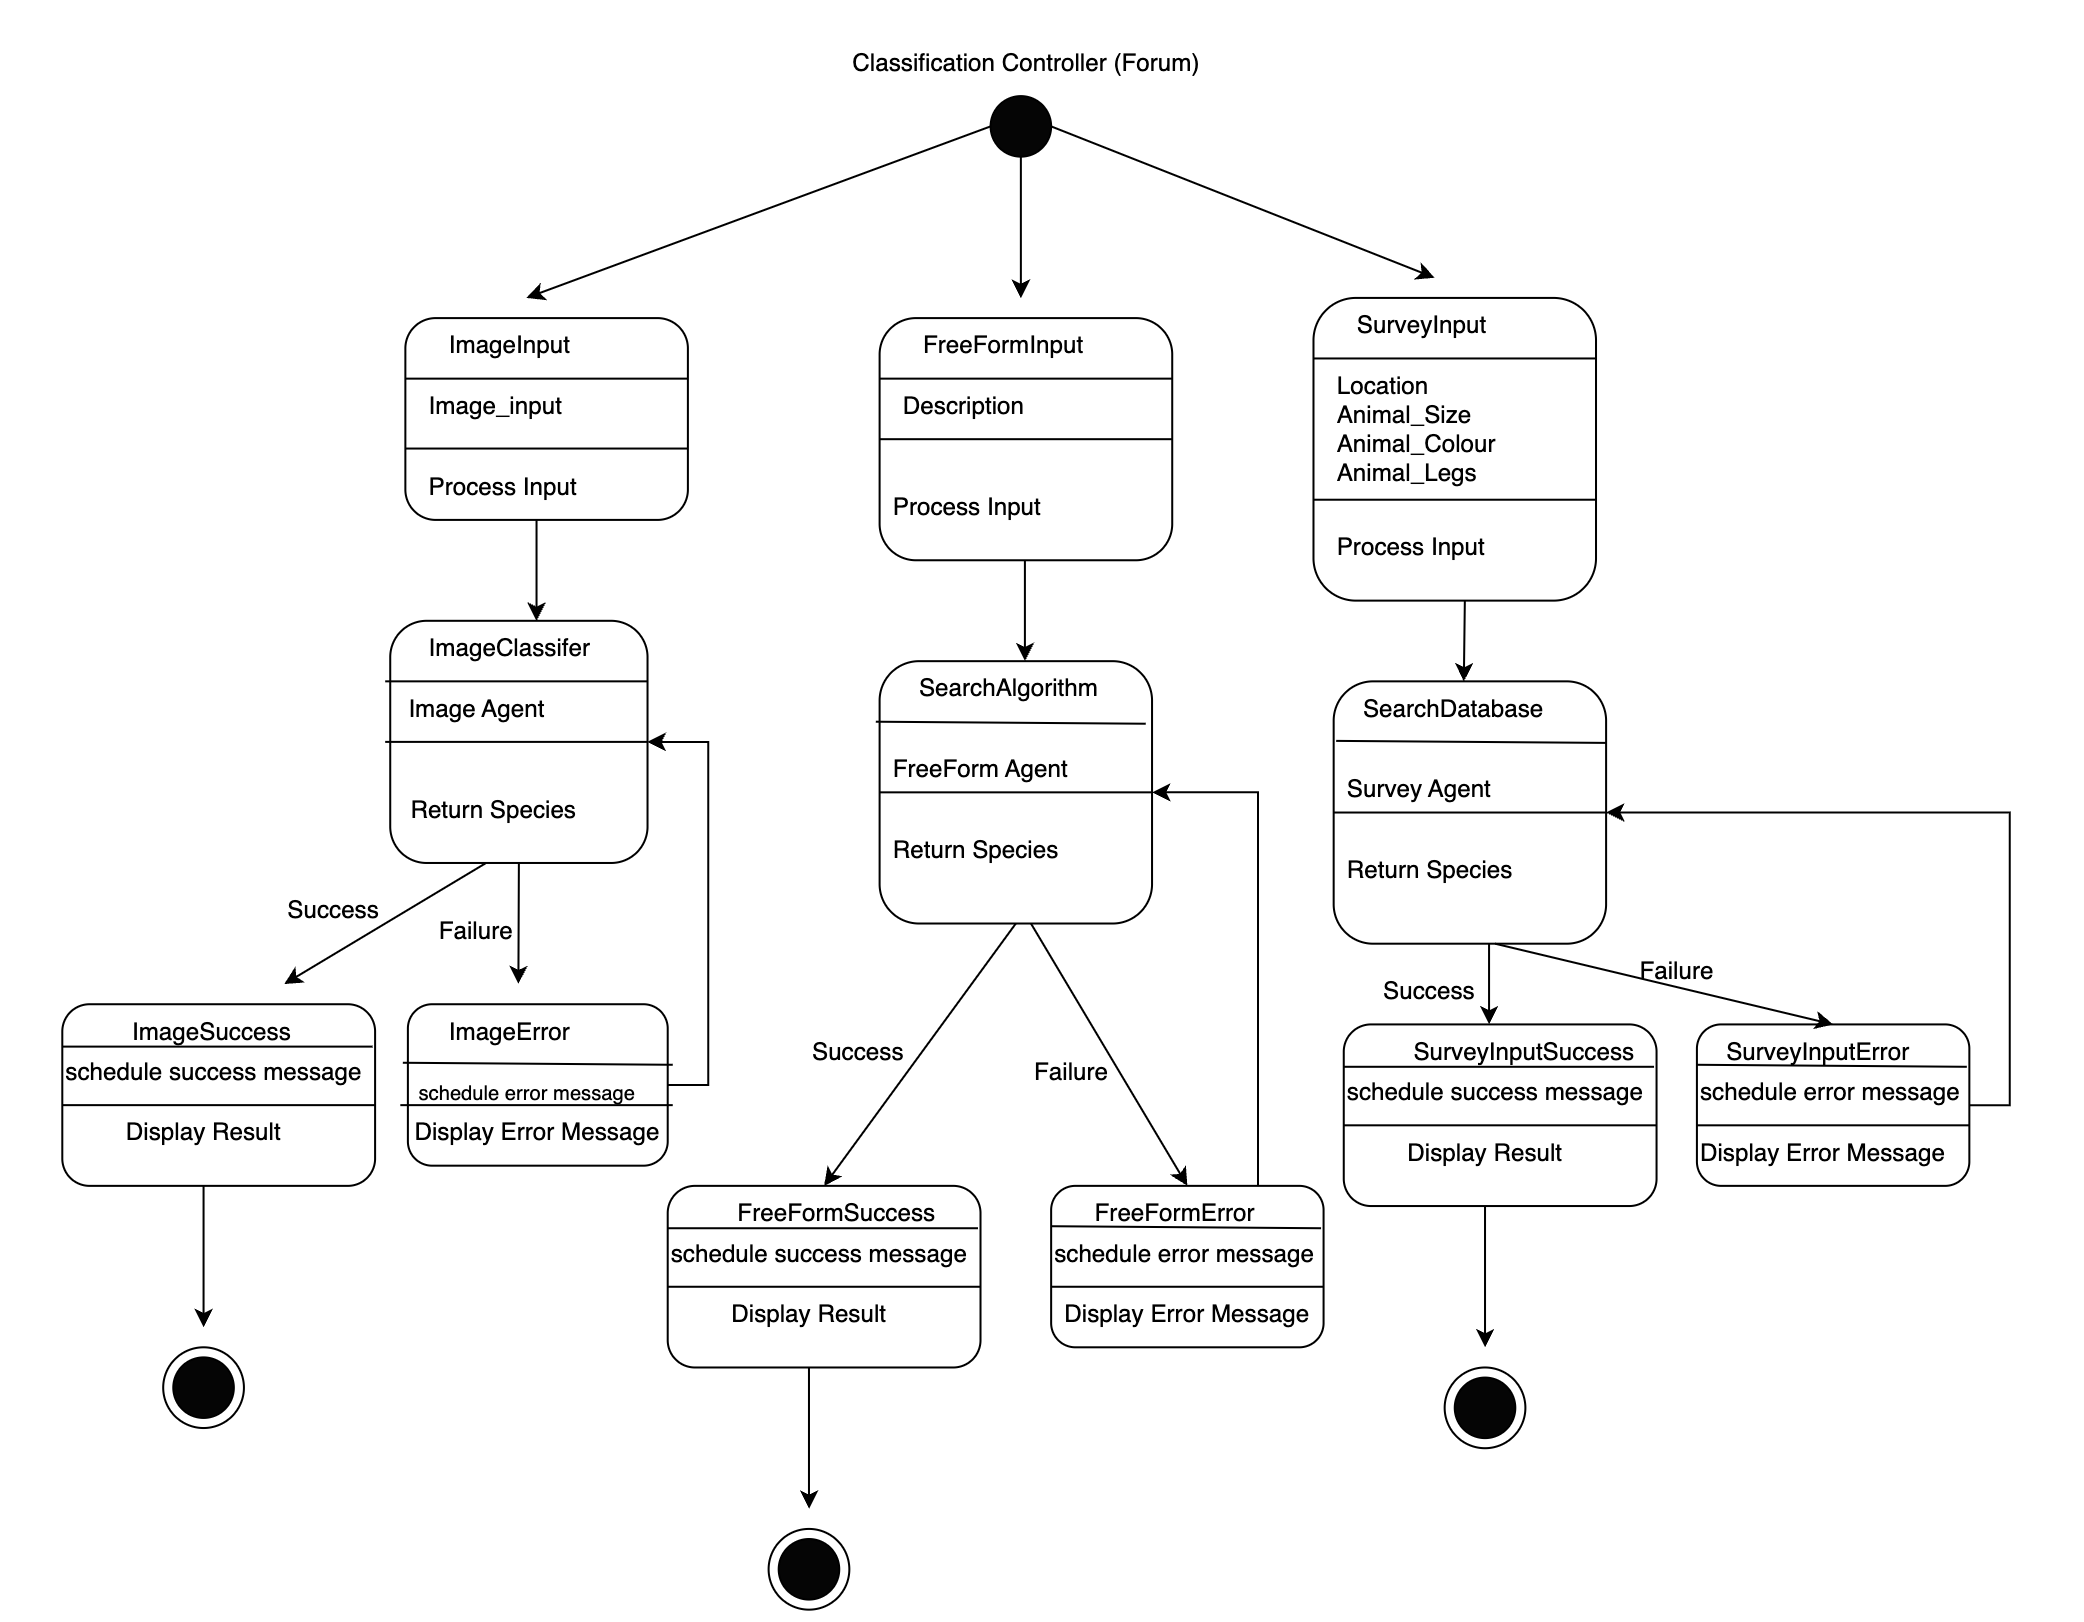
\includegraphics[scale=0.5]{Forum.png}
    \caption{Forum Controller State Chart Diagram}
    \label{fig:forum_controller}
\end{figure}
\clearpage 
\begin{figure}[h]
    \centering
    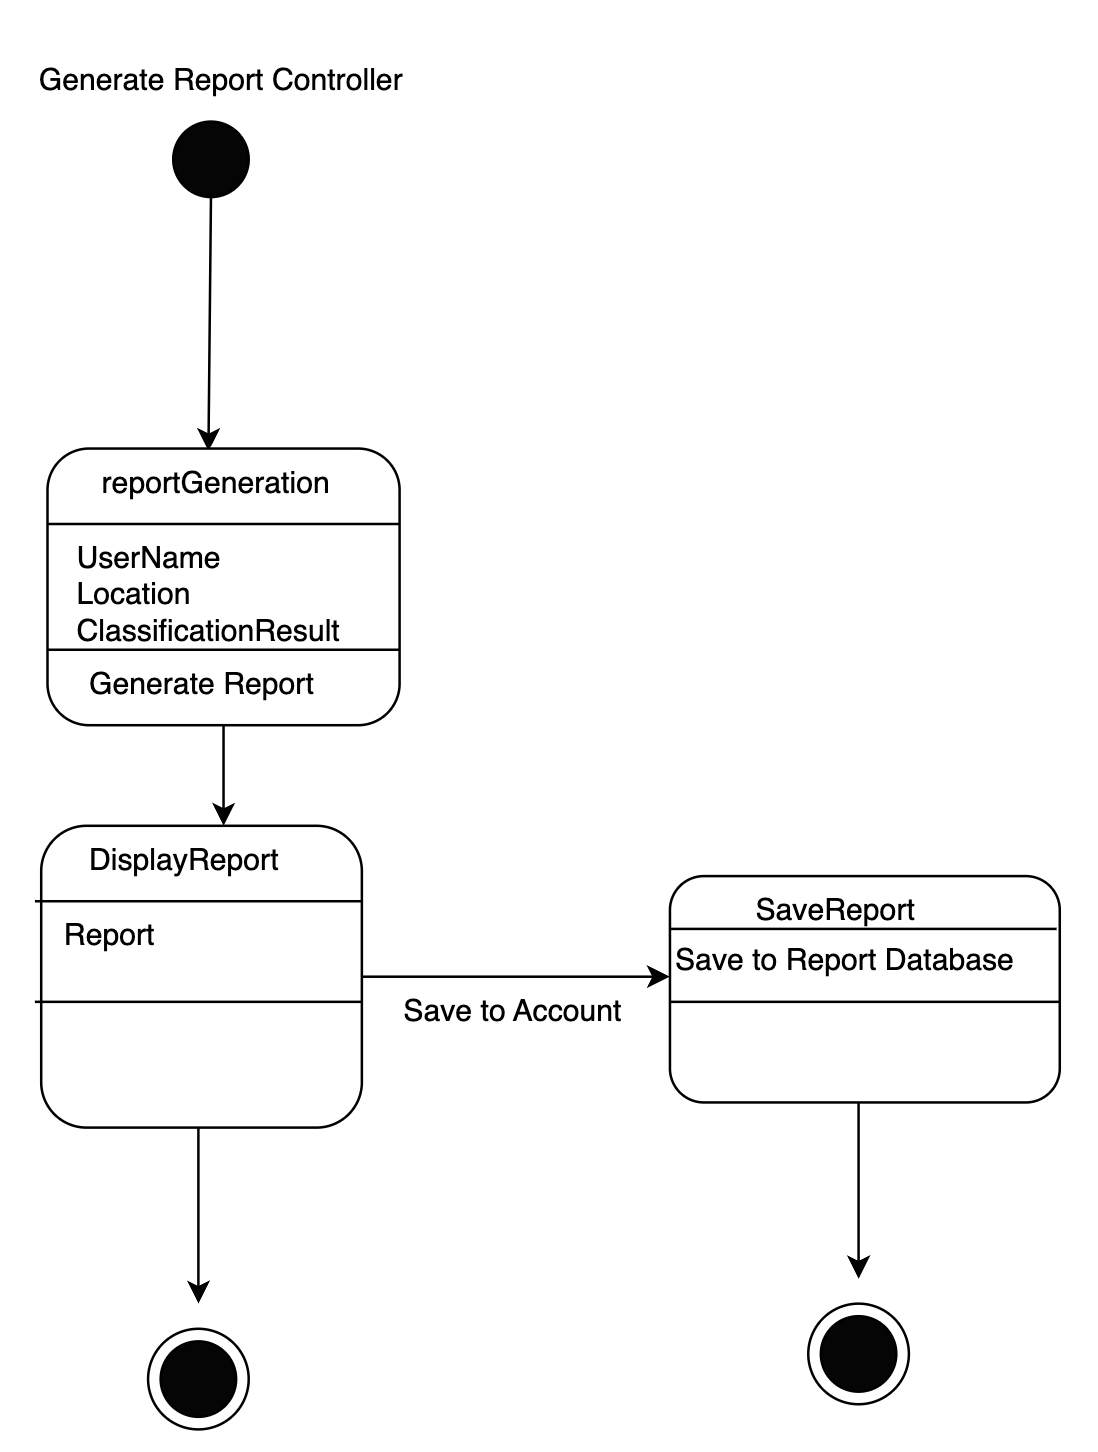
\includegraphics[scale=0.7]{GenerateReport.png}
    \caption{Generate Report Controller State Chart Diagram}
    \label{fig:generate_report_controller}
\end{figure}
\clearpage 
\begin{figure}[h]
    \centering
    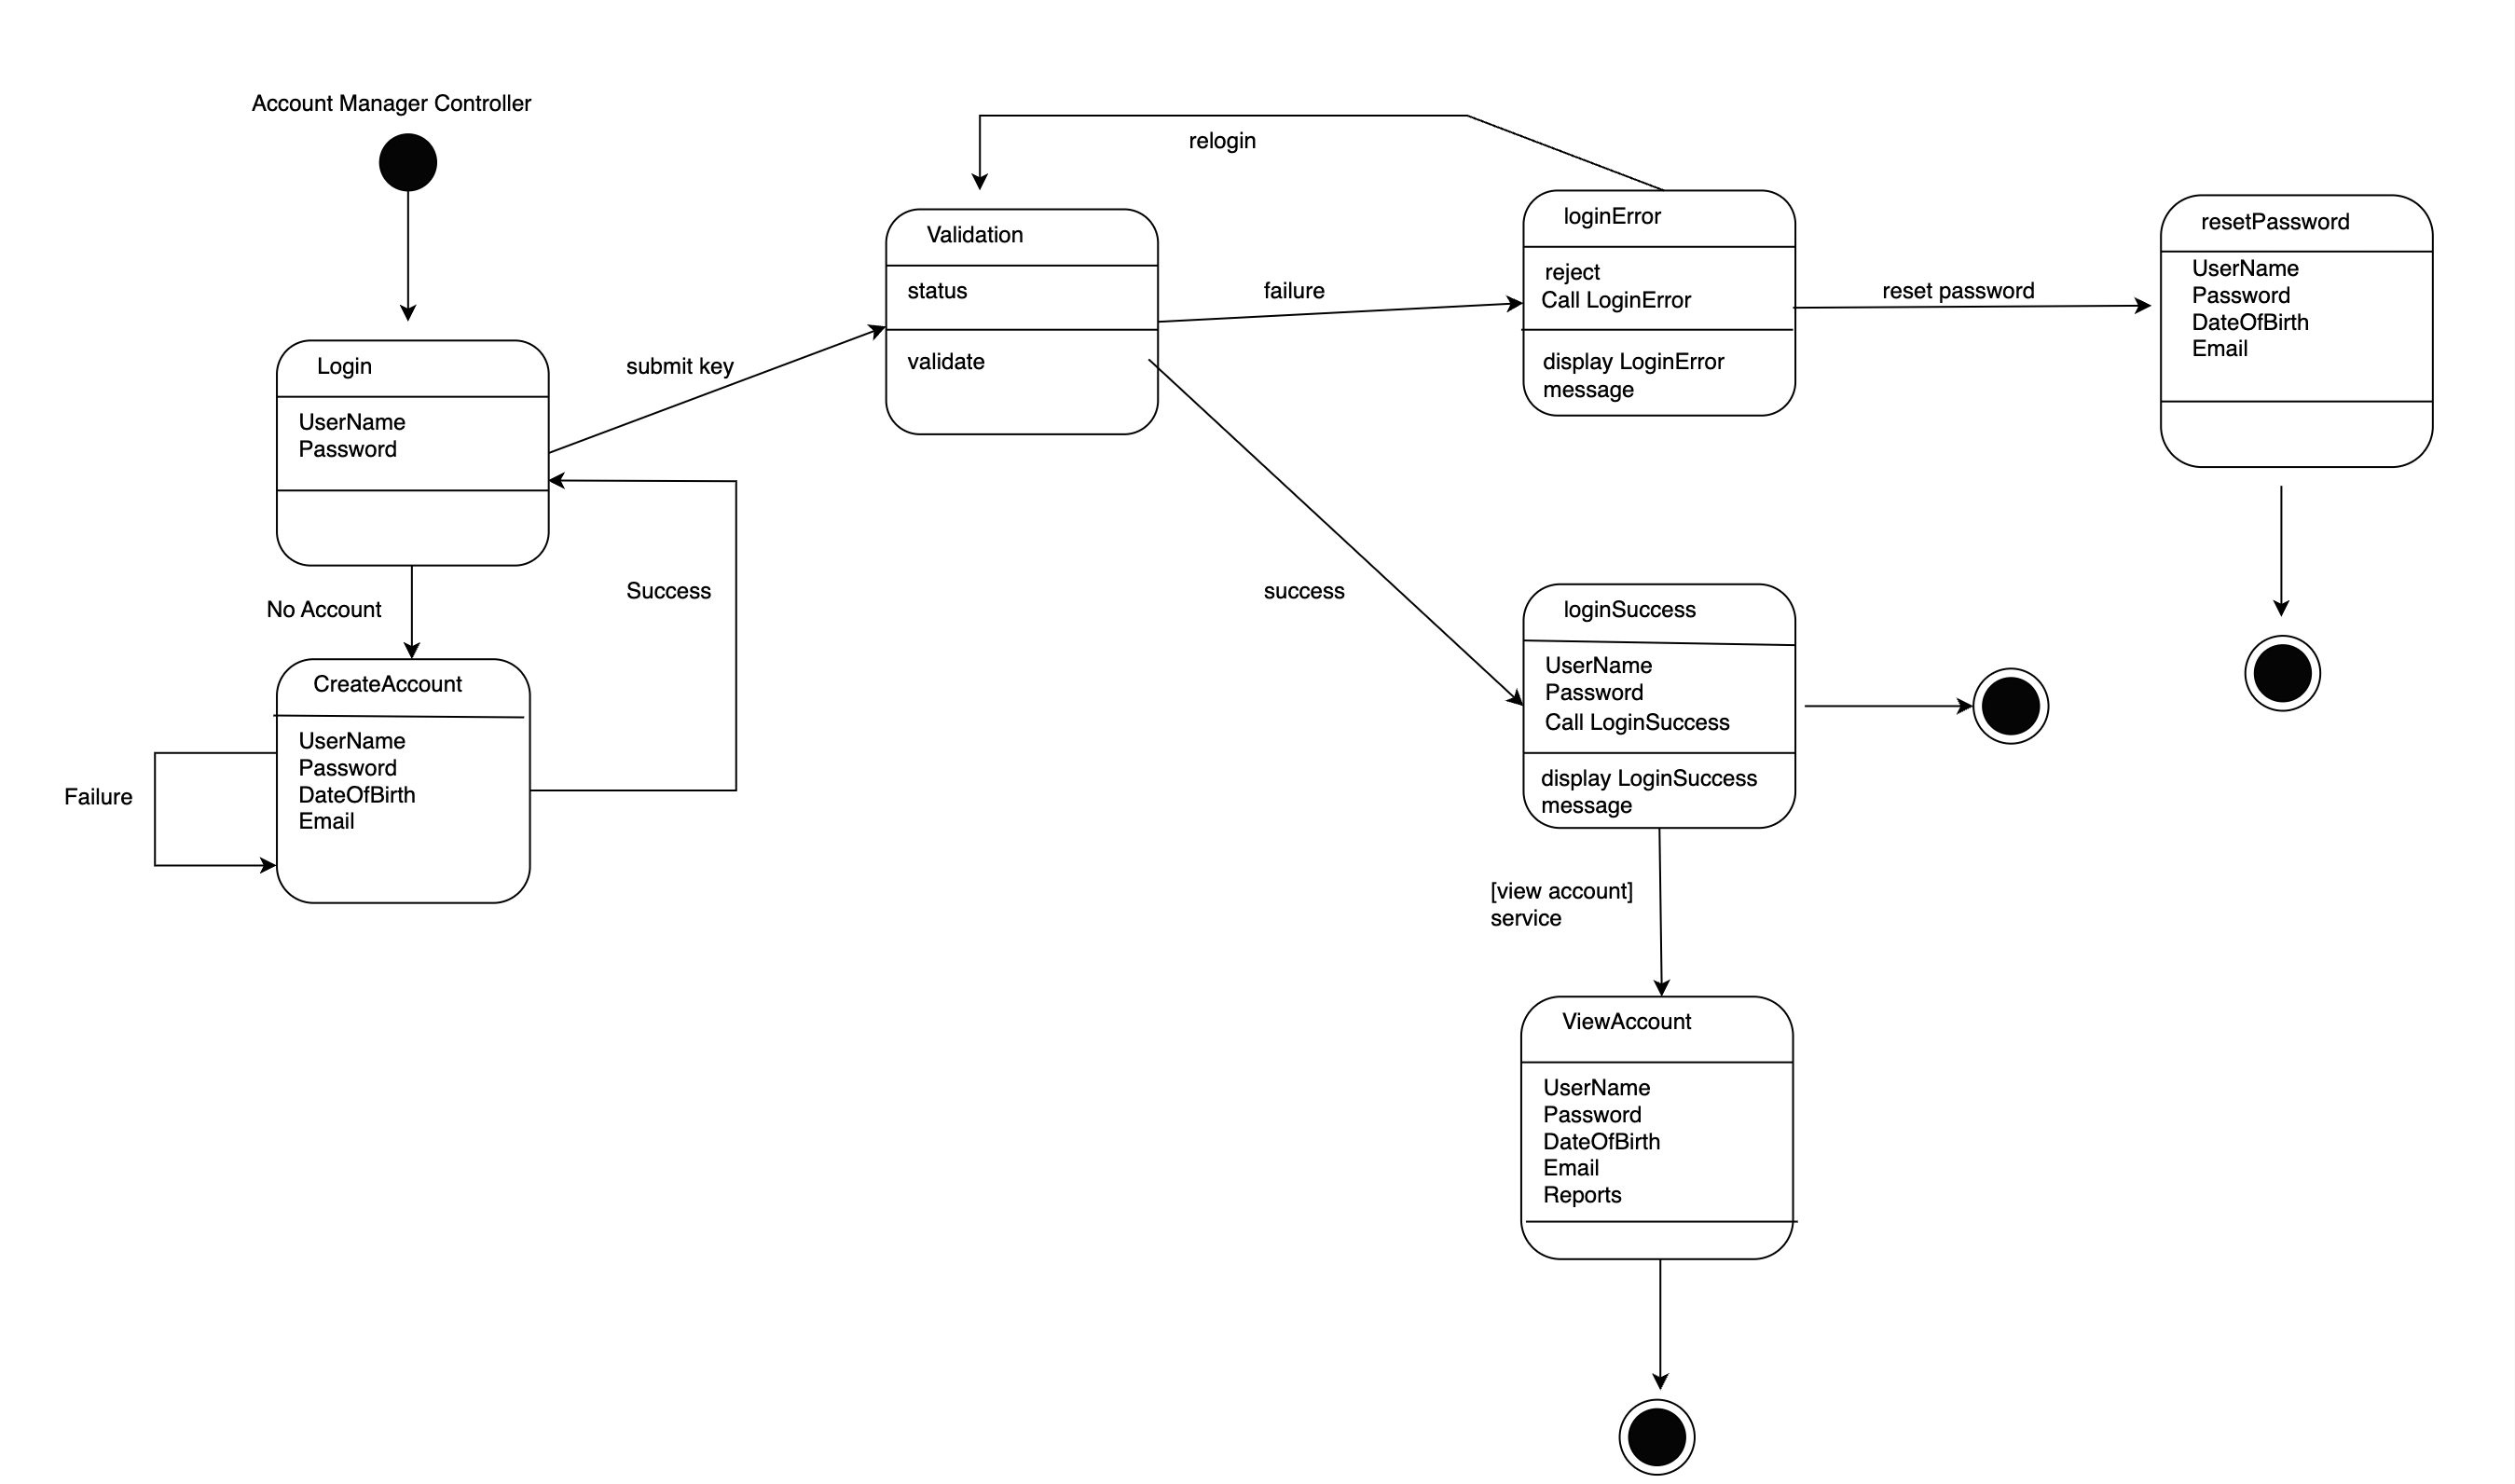
\includegraphics[scale=0.4]{AccountManager.png}
    \caption{Account Manager Controller State Chart Diagram}
    \label{fig:account_manager_controller}
\end{figure}
\clearpage 
\begin{figure}[h]
    \centering
    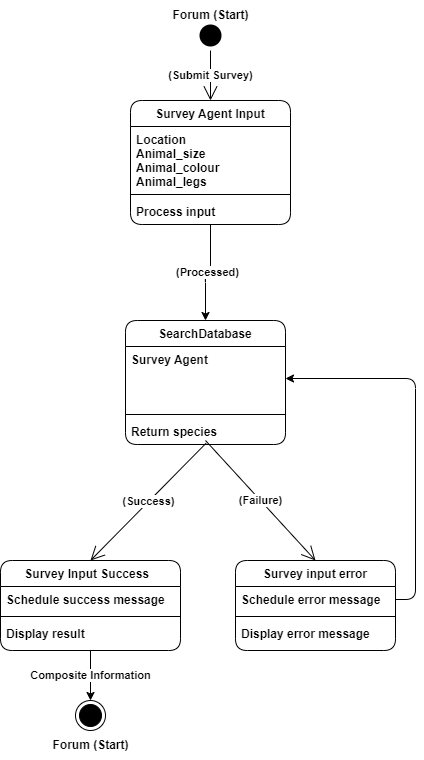
\includegraphics[scale=0.8]{Survey_Agents.png}
    \caption{Account Manager Controller State Chart Diagram}
    \label{fig:account_manager_controller}
\end{figure}
\clearpage 
\begin{figure}[h]
    \centering
    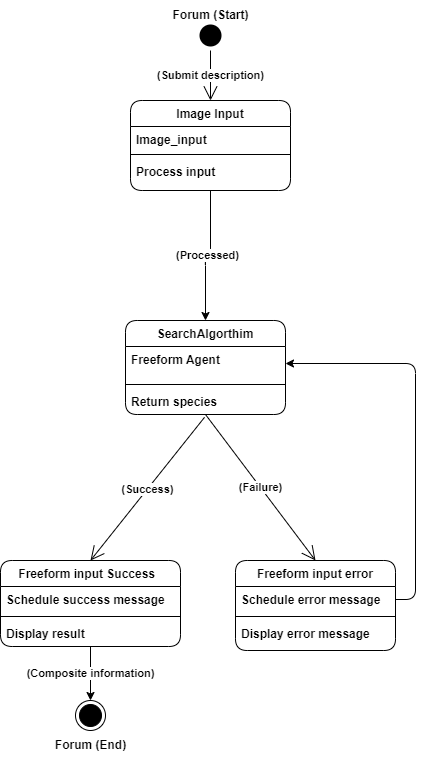
\includegraphics[scale=0.8]{FreeForm_Agent.png}
    \caption{Account Manager Controller State Chart Diagram}
    \label{fig:account_manager_controller}
\end{figure}
\clearpage 
\begin{figure}[h]
    \centering
    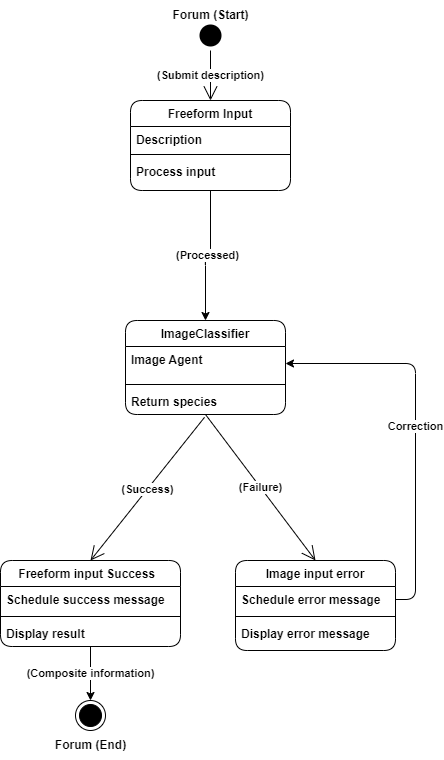
\includegraphics[scale=0.8]{Image_Agent.png}
    \caption{Account Manager Controller State Chart Diagram}
    \label{fig:account_manager_controller}
\end{figure}

\clearpage 

% End Section

\section{Sequence Diagrams}
\label{sec:sequence_diagrams}
\begin{figure}[h]
    \centering
    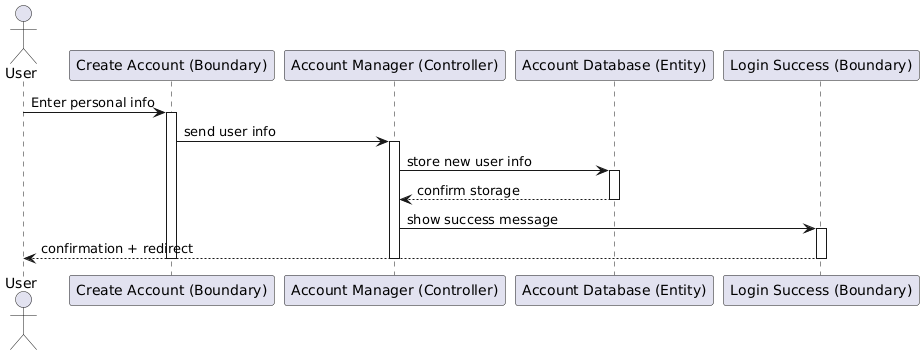
\includegraphics[scale=0.5]{login_sequence.png}
    \caption{Log in to Account Sequence Diagram}
    \label{fig:login_sequence}
\end{figure}
\clearpage

\begin{figure}[h]
    \centering
    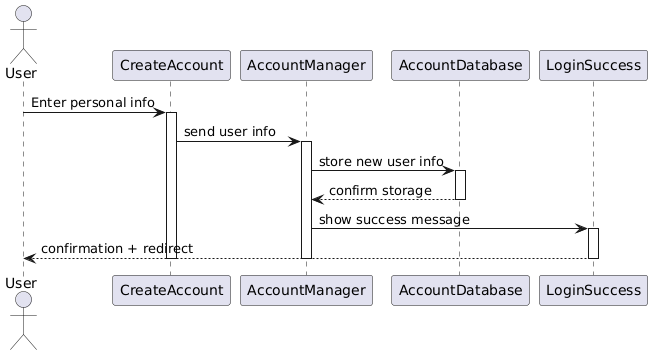
\includegraphics[scale=0.7]{CreateAccount_sequence.png}
    \caption{Creating an Account Sequence Diagram}
    \label{fig:CreateAccount_sequence}
\end{figure}
\clearpage

\begin{figure}[h]
    \centering
    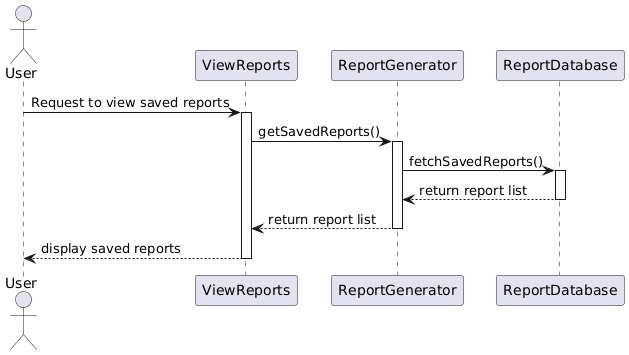
\includegraphics[scale=0.7]{ViewSavedReports_sequence.png}
    \caption{Viewing a Saved Report Sequence Diagram}
    \label{fig:ViewSavedReports_sequence}
\end{figure}
\clearpage

\begin{figure}[h]
    \centering
    \includegraphics[scale=0.7]{ImageSearch_sequence.png}
    \caption{Start Image Search Sequence Diagram}
    \label{fig:ViewSavedReports_sequence}
\end{figure}
\clearpage


\begin{figure}[h]
    \centering
    \includegraphics[scale=0.7]{FreeFormSearch_sequence.png}
    \caption{Start Freeform Text Search Sequence Diagram}
    \label{fig:ViewSavedReports_sequence}
\end{figure}
\clearpage

\begin{figure}[h]
    \centering
    \includegraphics[scale=0.7]{SurveySearch_sequence.png}
    \caption{Start Survey Search Sequence Diagram}
    \label{fig:ViewSavedReports_sequence}
\end{figure}
\clearpage

\section{Detailed Class Diagram}
\label{sec:detailed_class_diagram}
% Begin Section
This section should provide a detailed class diagram for your application.
% End Section

\appendix
\section{Division of Labour}
\label{sec:division_of_labour}
% End Section

% \newpage
% \section*{IMPORTANT NOTES}
% \begin{itemize}
% 	\item You do \underline{NOT} need to provide a text explanation of each diagram; the diagram should speak for itself
% 	\item Please document any non-standard notations that you may have used
% 	\begin{itemize}
% 		\item \emph{Rule of Thumb}: if you feel there is any doubt surrounding the meaning of your notations, document them
% 	\end{itemize}
% 	\item Some diagrams may be difficult to fit into one page
% 	\begin{itemize}
% 		\item It is OK if the text is small but please ensure that it is readable when printed
% 		\item If you need to break a diagram onto multiple pages, please adopt a system of doing so and throughly explain how it can be reconnected from one page to the next; if you are unsure about this, please ask me
% 	\end{itemize}
% 	\item Please submit the latest version of Deliverable 1 and Deliverable 2 with Deliverable 3
% 	\begin{itemize}
% 		\item They do not have to be a freshly printed versions; the latest marked versions are OK
% 	\end{itemize}
% 	\item If you do \underline{NOT} have a Division of Labour sheet, your deliverable will \underline{NOT} be marked
% \end{itemize}


\textbf{Cass Braun}
\begin{itemize}
    \setlength\itemindent{2em}
    \item text

\includegraphics[width=0.6\textwidth]{Cass.jpg}
\end{itemize}

\textbf{Nehad Shikh Trab}
\begin{itemize}
    \setlength\itemindent{2em}
    \item Section 3 - Log in to account Sequence Diagram
    \item Section 3 - Creating an account Sequence Diagram
    \item Section 3 - Viewing saved reports Seqeucen Diagram
    \item Assisted with formatting
\end{itemize}

\includegraphics[width=0.6\textwidth]{Nehad.png}
\\
\textbf{Savvy Liu}
\begin{itemize}
    \setlength\itemindent{2em}
    \item Section 3 - Start Image Search Sequence Diagram
    \item Section 3 - Start Freeform Text Search Sequence Diagram
    \item Section 3 - Start Survey Search Sequence Diagram
    \item General formatting checks and proofreading
\end{itemize} 

\includegraphics[width=0.6\textwidth]{Savvy.png}
\\
\textbf{Tvesha Shah}
\begin{itemize}
    \setlength\itemindent{2em}
    \item Section 2 - Forum Controller State Diagram 
    \item Section 2 - Account Manager Controller State Diagram 
    \item Section 2 - Generate Report Controller State Diagram 
    \item Section 1.1 Purpose
    \item Section 1.2 System Description
    \item Section 1.3 Overview
    \item Managed github set up and assisted with formatting
\end{itemize} 
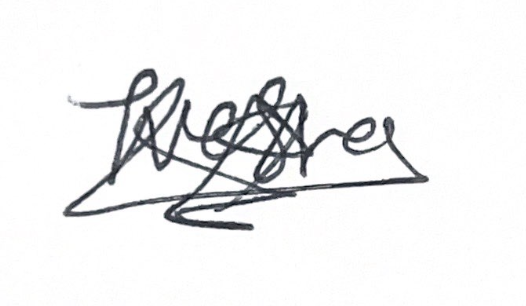
\includegraphics[width=0.6\textwidth]{Tvesha.png}
\\
\textbf{Victor Yu}
\begin{itemize}
    \setlength\itemindent{2em}
    \item Section 2 - Survey Agent State Diagram 
    \item Section 2 - Image Agent State Diagram 
    \item Section 2 - Freeform diagram State Diagram 
    \item Assisted with formatting, Forum State Diagram
\end{itemize} 

\includegraphics[width=0.3\textwidth]{Victor.png}
% End Section

\end{document}
%------------------------------------------------------------------------------